\documentclass[handout,10pt]{beamer}
\usepackage{SexySlides1,fancyvrb,outlines,pbox}

\definecolor{UniBlue}{RGB}{83,121,170}
\setbeamercolor{title}{fg=UniBlue}
\setbeamercolor{frametitle}{fg=UniBlue}
\newcommand{\colubf}{\color{UniBlue} \bf}

%% smart verbatim
\fvset{framesep=1cm,fontfamily=courier,fontsize=\scriptsize,framerule=.3mm,numbersep=1mm,commandchars=\\\{\}}

\title[Envelopes in Chemometrics]
{\Large  
Modeling Mutagenicity Status\\of a Diverse Set of Chemical Compounds\\by Envelope Methods
}

\author[]
{Subho Majumdar}

\institute[]
{School of Statistics, University of Minnesota} 

\date [August 4, 2014]

%%%%%%%List Outline in the beginning of each section.
\AtBeginSection[] {
   \begin{frame}
       \frametitle{Outline}
       \tableofcontents[currentsection]
   \end{frame}
}

%-------------------------------------------------------------------
\begin{document}

%\begin{frame}
\frame{ \titlepage}
%\end{frame}

%---------------------------------------------------

\begin{frame}
\frametitle{Motivation}
\begin{itemize}
\item Predictive analysis of data in Chemistry
\vspace{.2cm}
\item Generation of \textit{in silico} models to predict activities of chemical compounds
\vspace{.2cm}
\item Application in drug development to reduce cost of manufacturing derivatives of chemicals
\vspace{.2cm}
\item {\colbbf Specific problem} Binary class prediction in heterogeneous multivariate data(e.g. mutagen/ non-mutagen, curative effect of drug): \textbf{dimension reduction}
\end{itemize}
\end{frame}

\frame{\frametitle{Table of contents}\tableofcontents}

\section{The data and the variables}

\begin{frame}
\frametitle{The data}
\begin{itemize}
\item The data were taken from the CRC Handbook of Identified Carcinogens and Non-carcinogens \cite{crc}.
\vspace{.2cm}
\item Response variable is 0/1 mutagen status obtained from \textit{Ames test of mutagenicity}. A chemical compound was classified as mutagen (scored 1) if its Ames score exceeded a certain cutoff, non-mutagen (scored 0) otherwise.
\vspace{.2cm}
\item Total 508 compounds- 256 mutagens and 252 non-mutagens.
\vspace{.2cm}
\item The dataset is diverse, meaning that chemical compounds belong to fairly different from each other, like Alkanes and Amines.
\end{itemize}
\end{frame}

\begin{frame}
\begin{figure}\begin{center}
   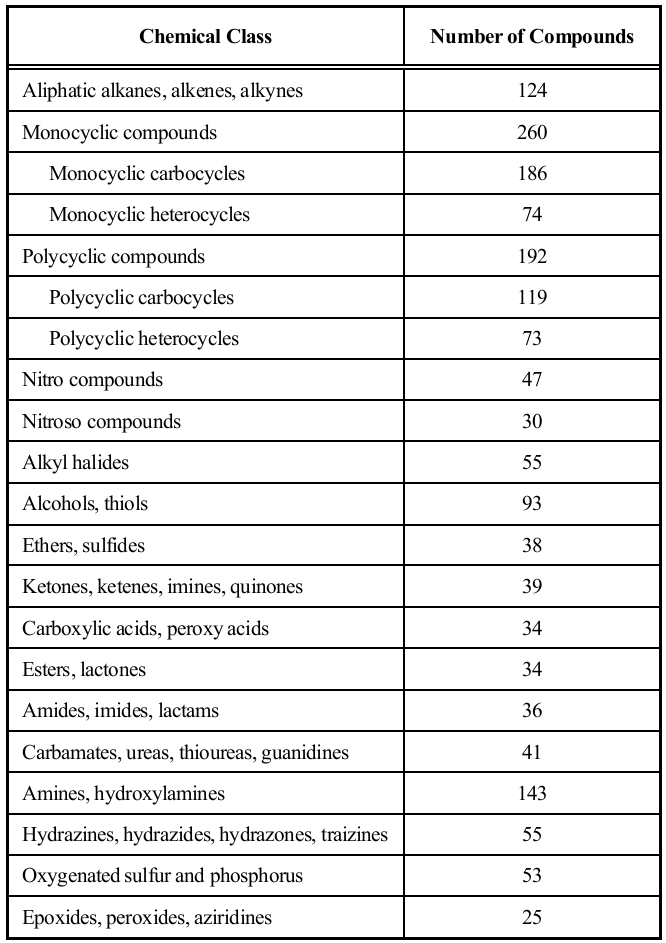
\includegraphics[height=8cm]{class.png}
   \label{fig:fig1}
\end{center}\end{figure}
\end{frame}

\begin{frame}
\frametitle{Description of variables}
Four types of variables:\vspace{.5cm}
\begin{enumerate}
\item \textbf{Topostructural (TS)}- Define the molecular topology, i.e. connectedness of atoms within a molecule (103 descriptors).
\vspace{.2cm}
\item \textbf{Topochemical (TC)}- Have information on atom and bond types (195 descriptors).
\vspace{.2cm}
\item \textbf{3-dimensional (3D)}- Define 3-dimensional aspects of the overall molecular structure (3 descriptors).
\vspace{.2cm}
\item \textbf{Quantum-Chemical (QC)}- Electronic aspects of molecular structure (6 descriptors).
\end{enumerate}
\end{frame}

\begin{frame}
\frametitle{Previous work}
\begin{itemize}
\item Use of {\colbbf Ridge Regression} to build a predictive model of mutagenicity \cite{hawk}. The 0/1 mutagenicity score was used as response variable since 1 corresponds to a higher mutagenicity score and 0 corresponds to a lower one.
\vspace{0.5cm}
\item {\colbbf Variable selection} on a larger set of predictors by adapting a supervised clustering algorithm previously used on high-dimensional genetic data \cite{majum}.
\end{itemize}
\end{frame}

\section{The models}

\begin{frame}
\frametitle{Envelope regression model}

$$ \bfY_i = \bfalpha + \bfbeta\bfX_i + \bfepsilon_i,\quad \bfepsilon_i\sim N(\bfZero,\bfSigma) \mbox{ with }\bfSigma = \bfGamma\bfOmega\bfGamma^T + \bfGamma_0\bfOmega_0\bfGamma_0^T$$
$$ i = 1,2,...,n $$
\begin{itemize}
\item Due to {\colubf Cook, Li and Chiaromonte, 2010} \cite{cook}.
\vspace{.2cm}
\item $\bfY\in\BR^{r\times n}$ multivariate response vector, $\bfX\in\BR^{p\times n}$ \textit{non-stochastic predictors}.
\item $\bfalpha\in\BR^r$ intercept, $\bfbeta\in\BR^{r\times p}$ matrix of regression coefficients: both unknown.
\item $\bfGamma\in\BR^{r\times u},\bfGamma_0\in\BR^{r\times (r-u)}$ semi-orthogonal basis matrices of $\cE_\bfSigma(\cB)$ and its orthogonal complement, respectively, with $\cB = \mbox{span}(\bfbeta)$ and $0\leq u\leq r$ being the dimension of the envelope.
\item $\bfOmega = \bfGamma\bfSigma\bfGamma^T, \Omega_0 = \bfGamma_0\bfSigma\bfGamma_0^T$ coordinate matrices corresponding to $\bfGamma, \bfGamma_0$.
\end{itemize}
\end{frame}

\begin{frame}
\frametitle{Graphical illustration of envelope model}
\begin{figure}\begin{center}
   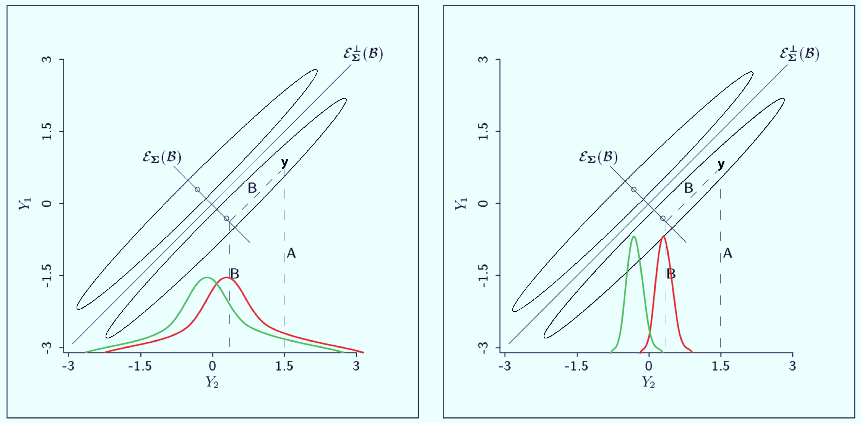
\includegraphics[height=5cm]{env.png}
   \label{fig:fig1}
\end{center}\end{figure}
\begin{center}
{\colubf (Source: Stat 8932 class notes, R. Dennis Cook)}
\end{center}
\end{frame}

\begin{frame}
\frametitle{Envelope regression model for our data: basics}
\begin{itemize}
\item log-transformed data.
\vspace{.2cm}
\item Predictors taken as multivariate response, and the 0/1 mutagenicity status taken as the single predictor, and then envelope regression models are obtained.
\vspace{.2cm}
\item Hierarchical approach to observe the effect of adding different classes of predictors: separate envelope models fit on data with only TS, only TC, TC + TS and full set of predictors.
\vspace{.2cm}
\item Data rank deficient, so PCA was performed on data and envelope model was built on first few PCs that explained 90\% (or 95\%) of total variation.
\end{itemize}
\end{frame}

\begin{frame}
\frametitle{Supervised Singular-Value Decomposition (SupSVD)}
$$ \bfX = \bfY\bfB\bfV^T + \bfF\bfV^T + \bfE $$
\begin{itemize}
\item Due to {\colubf Li et al, 2014} \cite{supsvd}.
\vspace{.2cm}
\item  Matrix of predictors $\bfX\in\BR^{n\times p}$, supervision data matrix $\bfY\in\BR^{n\times r}$.
\vspace{.2cm}
\item $\bfB\in\mathbb{R}^{r\times q}$ is the multivariate matrix of coefficients, $\bfV\in\mathbb{R}^{p\times q}$ full-rank loading matrix.
\vspace{.2cm}
\item $0\leq q\leq r$ the dimension of the underlying space of latent parameters, and $\bfF\sim\mathcal{N}_q(\bf0,\bfSigma_f), \bfE\sim\mathcal{N}_p(\bf0,\sigma_e^2\bfI_p)$ are random error matrices s.t. $\bfSigma = \bfV\bfSigma_f\bfV^T + \sigma_e^2\bfI_p$.
\vspace{.2cm}
\item A modified EM algorithm is used to obtain the unknown parameters $\bftheta=(\bfB,\bfV,\bfSigma_f,\sigma_e^2)$.
\vspace{.2cm}
\item The vector of mutagenicity status is now used as the supervision data matrix $\bfY$, while the data on 308 predictors is the matrix $\bfX$.
\end{itemize}
\end{frame}

\begin{frame}
\frametitle{Prediction through Linear Discriminant Analysis}
\begin{itemize}
\item \textbf{Envelope model}- Estimate the envelope basis, say $\hat\bfGamma$, reduce the matrix of predictors by multiplying it with the basis and then apply Fisher's Linear Discriminant Analysis on $\hat\bfGamma^T\bfY$.
\vspace{.2cm}
\item \textbf{supSVD}- Here the notations are reversed and $\bfX$ is our $508\times 307$ data matrix. After obtaining the loading matrix $\bfV$, we transform the data matrix as: $\bfU = \bfX\bfV$, and apply LDA on $\bfU$, taking $\bfY$ as the 0/1 class variable.
\vspace{.2cm}
\item Correct classification percentages are obtained through cross-validation
on the full sample.
\end{itemize}
\end{frame}

\begin{frame}
\frametitle{Method of Cross-validation}
\begin{center}\begin{large}
{\colubf Na\"{i}ve CV vs. Two-fold CV}
\end{large}\end{center}
\begin{figure}\begin{center}
   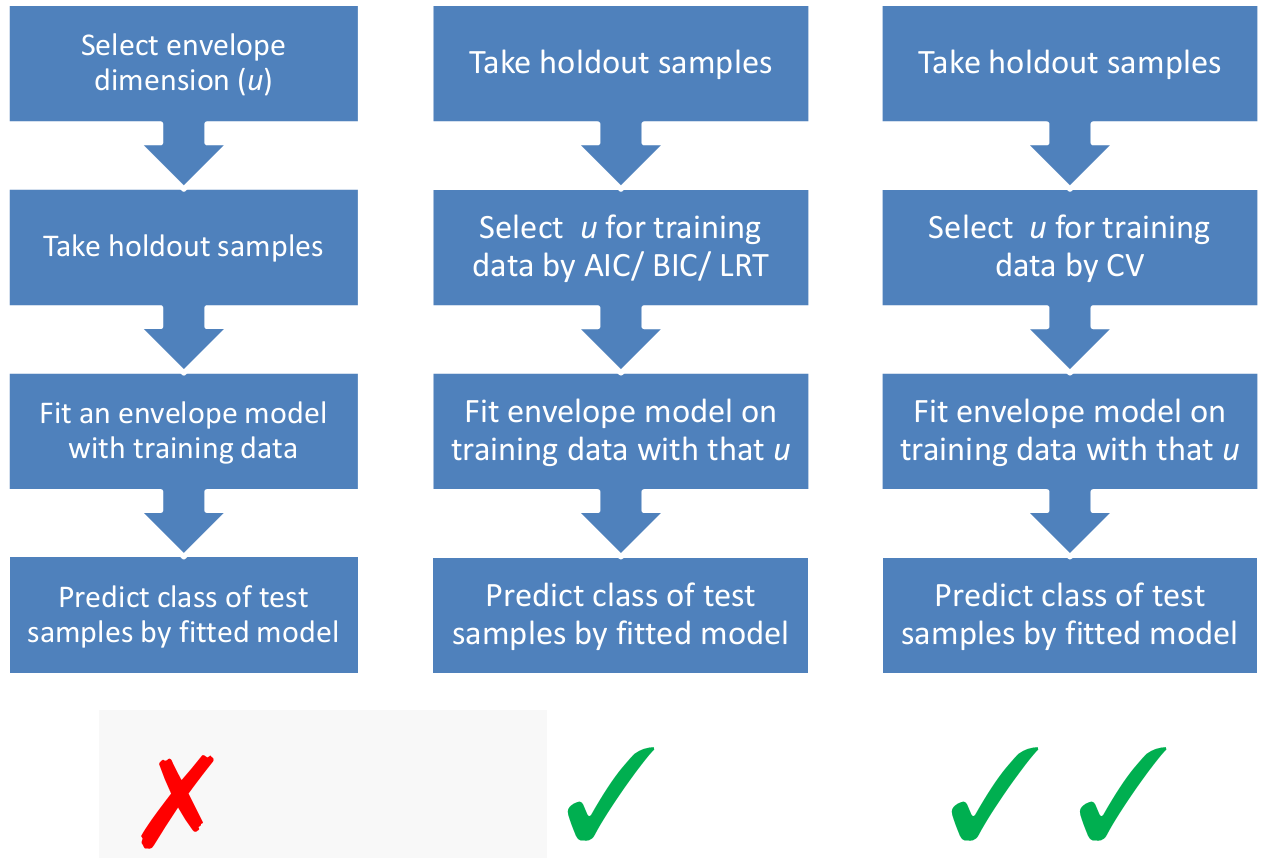
\includegraphics[height=7cm]{cv.png}
   \label{fig:fig2}
\end{center}\end{figure}
\end{frame}

\section{Results}
\begin{frame}
\frametitle{Results: Variance reduction by envelopes}
In all the envelope models, there were massive gains in terms of variation. The gains were especially large for the first 2 principal components.
\vspace{.2cm}

\begin{scriptsize}
\begin{table}\centering
    \begin{tabular}{|c|c|c||c|c|c|c|c|c|}\hline
    \textbf{Set of} & \textbf{No. of} & \textbf{Envelope} & 
    \multicolumn{3}{c|}{\textbf{\% variance explained by}} & \multicolumn{3}{c|}{\textbf{Envelope gain ratios for}}\\\cline{4-9}
    \textbf{descriptors}                  & \textbf{PCs}                                                 & \textbf{dimension} ($u$) & \textbf{PC1}                      & \textbf{PC2}   & \textbf{PC3}  & \textbf{PC1}                & \textbf{PC2}   & \textbf{PC3}  \\\hline\hline
    \textbf{TS}                 & 7                                                 & 3                        & 70.43                    & 10.35 & 2.60 & 25.91              & 36.17 & 2.10 \\ \hline
    \textbf{TC}                 & 8                                                 & 4                        & 75.89                    & 6.52  & 2.42 & 15.40              & 35.26 & 1.00 \\\hline
    \textbf{TS + TC}            & 13                                                & 6                        & 70.27                    & 7.94  & 2.21 & 10.40              & 37.99 & 1.22 \\\hline
    \textbf{Full} & 15 & 11 & 58.19 & 7.60 & 5.98 & 1.00 & 1.00 & 1.00 \\\hline
    \end{tabular}
\end{table}
\end{scriptsize}
\vspace{.2cm}
\textbf{Note}:
\begin{itemize}
\item With default tolerances of objective and gradient function in \texttt{env} the algorithm did not converge in 1000 iterations. For this reason they were set to \texttt{1e-7} and \texttt{1e-4}.
\vspace{.2cm}
\item As far as other PCs of full model were concerned, PCs 9, 11, 13 and 15 gave 1.26, 1.96, 1.88 and 1.5-fold gains, respectively.
\end{itemize}
\end{frame}

\begin{frame}
\frametitle{Performance of envelopes and supSVD in prediction}
\begin{scriptsize}
\begin{table}[t]\centering
    \begin{tabular}{|c|c|c|c|c|c|}
    \hline
    \textbf{Model}                                     & \textbf{Type of predictors} & \textbf{No. of}     & \multicolumn{3}{c|}{\textbf{Correct classification} \%}\\\cline{4-6}
    \textbf{description}                               & \textbf{in model}           & \textbf{predictors} & \quad\textbf{Total}  \quad                   & \textbf{Mutagens} & \textbf{Non-mutagens} \\ \hline
    Ridge regression\cite{hawk}                          & TS+TC              & 298        & \textbf{76.97}                     & \textbf{83.98}    & \textbf{69.84}        \\ \hline
    Ridge regression\cite{hawk}                          & TS+TC+3D+QC        & 307        & \textbf{77.17}                     & \textbf{84.38}    & \textbf{69.84}        \\ \hline
    \pbox{10cm}{Ridge regression after \\variable selection\cite{majum}} & TS+TC+AP           & 203        & \textbf{78.35}                     & \textbf{84.38}    & \textbf{72.22       } \\ \hline\hline
                                  & TS                 & 103        & {\colrbf 57.09}                     & {\colrbf 65.63}    & {\colrbf 48.41}        \\\cline{2-6}
    Envelope LDA                                         & TC                 & 195        & {\colrbf 58.27}                     & {\colrbf 69.92}    & {\colrbf 46.43}        \\\cline{2-6}
    ~                                         & TS+TC              & 298          & {\colrbf 60.24} & {\colrbf 69.14}        & {\colrbf 51.19}            \\ \hline\hline
     & TS & 103 (5) & {\colbbf 59.45} & {\colbbf 70.31} & {\colbbf 48.41} \\\cline{2-6}
  SupSVD LDA   & TC & 195 (37) & {\colbbf 70.47} & {\colbbf 76.56} & {\colbbf 64.29} \\\cline{2-6}
  90\% cutoff  & TS+TC & 298 (32) & {\colbbf 68.90} & {\colbbf 75.39} & {\colbbf 62.30} \\\cline{2-6}
    & TS+TC+3D+QC & 307 (34) & {\colbbf 70.47} & {\colbbf 77.73} & {\colbbf 63.09} \\\hline\hline
    
     & TS & 103 (8) & {\colbbf 60.04} & {\colbbf 67.58} & {\colbbf 52.38} \\\cline{2-6}
  SupSVD LDA & TC & 195 (51) & {\colbbf 72.44} & {\colbbf 78.13} & {\colbbf 66.67} \\\cline{2-6}
  95\% cutoff  & TS+TC & 298 (48) & {\colbbf 70.47} & {\colbbf 78.91} & {\colbbf 61.90} \\\cline{2-6}
    & TS+TC+3D+QC & 307 (51) & {\colbbf 71.06} & {\colbbf 78.91} & {\colbbf 63.09} \\\hline
    \end{tabular}
    \caption{Comparison of predictive performance of various models}
\end{table}

\end{scriptsize}
\end{frame}

\section{Conclusion}

\begin{frame}
\frametitle{Discussion}
\begin{outline}
\1 For estimation, envelope models performed really well in conjunction with PCA for rank-deficient data, offering heavy gains for the major principal components over OLS.
\vspace{.2cm}
\1 Possible reason for the poor performance in prediction:
\2 High material to immaterial variation ratio
\2 Heteroskedasticity caused by diverse chemical classes among compounds
\2 Variation of scales between different types of variables
\vspace{.2cm}
\1 Logistic Envelope Regression.
\vspace{.2cm}
\1 supSVD a potential plausible approach because of its general framework and computational stability and applicability in $n<<p$ scenario.
\end{outline}
\end{frame}

\begin{frame}
\frametitle{Acknowledgements}
\begin{itemize}
\item Prof. Dennis Cook, for his guidance and valuable inputs.
\vspace{.2cm}
\item Henry Zhang, for providing his codes for logistic envelope regression.
\vspace{.2cm}
\item Greg Grunwald, UofM-Duluth for providing the dataset.
\end{itemize}
\end{frame}

\begin{frame}
\frametitle{References}
\begin{footnotesize}
\bibliographystyle{acm}
\bibliography{envchemo}
\end{footnotesize}
\end{frame}
%\begin{frame}
%\frametitle{Description of variables}
%The first 5 questions are concerned with drinking and driving, the next 5 with other drug use, and the last two with sexual behavior. Also, QN29, QN40, QN44 and QN57 have a time component.
%
%\begin{figure}\begin{center}
%   \includegraphics[height=6cm]{hw231.png}
%   \label{fig:fig1}
%\end{center}\end{figure}
%\vspace{.5cm}
%\end{frame}

%\begin{frame}[fragile]
%\frametitle{Proportion of positive responses for each question}
%For the sake of simplicity only those cases that were fully observed are used in the analysis. Using those cases, the proportion of respondents who answered yes to each of the 12 questions are found as below:
%\begin{block}{}
%\begin{Verbatim}
%> load(url("http://tinyurl.com/yrbs05-rda"))
%> len = dim(yrbs05)[1]
%> probs = 1-(apply(yrbs05[,1:12], 2, sum) - len)/len; probs
%\textbf{      QN29       QN34       QN11       QN40       QN42       QN45       QN48 }
%\textbf{0.15757455 0.12945048 0.11319438 0.25132143 0.28473123 0.08935873 0.08935873 }
%\textbf{      QN50       QN52       QN53       QN58       QN59 }
%\textbf{0.11917822 0.06053655 0.05953924 0.06891393 0.16814601 }
%\end{Verbatim}
%\end{block}
%\end{frame}

%\begin{frame}[fragile]
%\frametitle{Fitting a model of complete independence}
%Following are the estimated probabilities for all 12 questions. Note that they are same as the probabilities in the last section.
%\begin{columns}[c]
%\column{1.5in}
%\begin{block}{}
%\begin{Verbatim}
%$QN29
%           Pr(1)  Pr(2)
%class 1:  0.1576 0.8424
%
%$QN34
%           Pr(1)  Pr(2)
%class 1:  0.1295 0.8705
%
%$QN11
%           Pr(1)  Pr(2)
%class 1:  0.1132 0.8868
%
%$QN40
%           Pr(1)  Pr(2)
%class 1:  0.2513 0.7487
%
%$QN42
%           Pr(1)  Pr(2)
%class 1:  0.2847 0.7153
%
%$QN45
%           Pr(1)  Pr(2)
%class 1:  0.0894 0.9106
%
%\end{Verbatim}
%\end{block}
%
%\column{1.5in}
%\begin{block}{}
%\begin{Verbatim}
%$QN48
%           Pr(1)  Pr(2)
%class 1:  0.0894 0.9106
%
%$QN50
%           Pr(1)  Pr(2)
%class 1:  0.1192 0.8808
%
%$QN52
%           Pr(1)  Pr(2)
%class 1:  0.0605 0.9395
%
%$QN53
%           Pr(1)  Pr(2)
%class 1:  0.0595 0.9405
%
%$QN58
%           Pr(1)  Pr(2)
%class 1:  0.0689 0.9311
%
%$QN59
%           Pr(1)  Pr(2)
%class 1:  0.1681 0.8319
%\end{Verbatim}
%\end{block}
%\end{columns}
%\end{frame}

\begin{frame}
\centering\huge
\textcolor{UniBlue}{\textbf{THANK YOU!}}
\end{frame}

\end{document} 

